\subsection{Question 1}

\lstinputlisting[caption=Matlab Commands,showstringspaces=false,language=Matlab]{../find_vectors.m}

\newpage
\subsubsection{Part A}

\lstinputlisting[caption=Matlab Commands,showstringspaces=false,language=Matlab]{../q1_partA}

\subsubsection{Part B}

\lstinputlisting[caption=Matlab Commands,showstringspaces=false,language=Matlab]{../q1_partB}

\newpage
\subsection{Question 2}

\begin{figure}[th]
  \centering
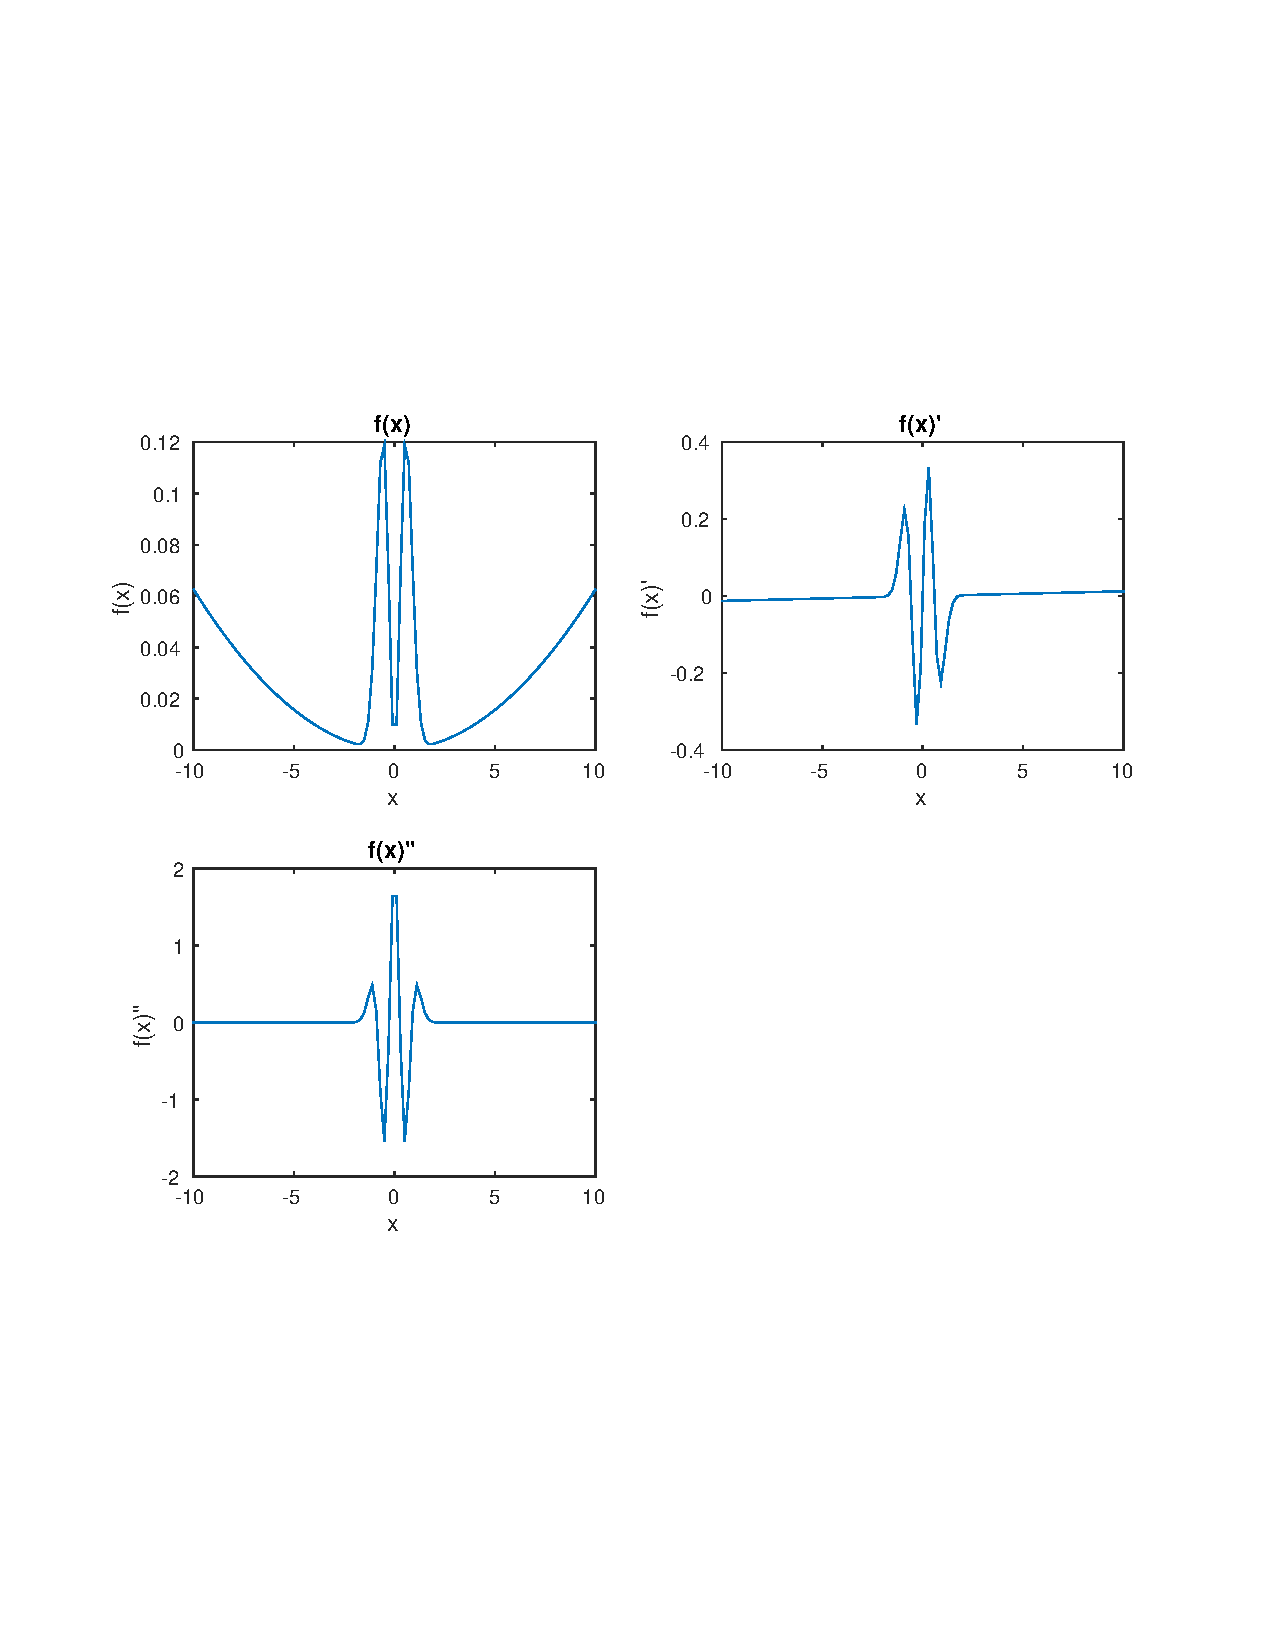
\includegraphics[trim=10mm 70mm 10mm 70mm, width=1.0\textwidth]{../q2_plots}
\end{figure}

\lstinputlisting[caption=Matlab Commands,showstringspaces=false,language=Matlab]{../q2_maxmin}

\newpage
\subsection{Question 3}
\subsubsection{Part C}
\subsubsection{Part D}
\subsubsection{Part E}

\newpage
\subsection{Question 4}
\subsubsection{Part A}
\subsubsection{Part B}
\subsubsection{Part C}

\newpage
\subsection{Question 5}
\subsubsection{Part A}
\subsubsection{Part B}
\subsubsection{Part C}
\subsubsection{Part D}

\newpage
\subsection{Question 6}

%\lstinputlisting[caption=Matlab Commands,showstringspaces=false,language=Matlab]{../q5_partC}
